\chapter{Introduction}
\label{ch:introduction}

All things start with Agile programming.
Since the writing of the agile manifesto\cite{AgileManifesto} in 2001, different practices have emerged.
Such practices include extreme programming, scrum, kanban and many more\cite{ADecadeOfAgileMethodologies}.
All of them with the goal of increasing the velocity of software development and the speed at which a project can change into different directions.
These agile practices are more and more adopted in the industry\cite{BecomingAgileTogether} and taught at universities\cite{StudienhandbuchProjectManagement}.

In recent years, however, a new set of practices emerged.
Expanding on agile practices, these have the same goal albeit with other means.
This set of practices is commonly referred to as ''DevOps'' practices.
A short summary, which is explored shortly, would be:

DevOps is IT for software developers.\footnote{A quote once overheard in passing.}

Ebert et.al.\ explain the field as an integration of two worlds\cite{DevOps}.
Automating both, development and operations.
Automating integration and delivery.
Automating testing and deploying.
Automating logging and monitoring.

The first need that arises to achieve this level of automation is the need for tools.
Again, Ebert et.al., as well as Leite et.al, identify this necessity\cite{DevOps, ASurveyofDevOpsConceptsandChallenges}.
First and foremost, build tools are required to automate building software systems.
Most of which also include some form of dependency management to automatically link required libraries to the resulting system.

Then, testing tools are required to automate testing newly integrated code and therefore streamline automatic integration.
Since this process is also called continuous integration, these tools are known as continuous integration tools\cite{DevOps}.
Closely related are the continuous delivery tools.
These satisfy the need of automatically delivering or deploying newly integrated code.
Usually, a tool that does continuous integration (CI) also does continuous delivery (CD) because of that fact.
They are then often called CI/CD tools for short.

Taking back a step, agile methods, as discussed in the beginning, have the goal of increasing the velocity of software development\cite{ADecadeOfAgileMethodologies}.
One of the principles these methods use to achieve this goal is the principle of collective code ownership\cite{CommonAgilePracticesInSoftwareProcesses, ManagingCodeOwnership}.
Until fairly recently, pipelines to automatically integrate and deliver code were often clicked together\cite{JenkinsClassicUi}.
As this practice slowly faded out, infrastructure as code emerged\cite{ASystematicMappingStudyOfInfrastructureAsCodeResearch}.
Since the infrastructure is now represented as code, it too can be collectively owned, enabling more DevOps practices and further increase development velocity.

Summarizing briefly, it is now established that automated pipelines exist and are used.
Their configuration is shared as pieces of code amongst members of a software team or other stakeholders.
They are used to automatically integrate code into a system and then deliver this system to customers.
It appears, as if these steps are logical and structured and that is indeed the case.
However, some details are still missing.

First, it must be discussed how to verify that the newly and automatically integrated code works well and as intended.
Secondly, where to deliver the system and how this can be done in a way, that is automatic as well as correctly.
After all, the system cannot just be put somewhere on the internet with the hopes that the customer will eventually figure out how to use the updated version.
Changelogs, version bumps, installation instructions and more must be carefully considered.
As this paper will show,  automating the maintenance of this secondary information must be done in a thoughtful and precise manner.

\begin{figure}[H]
\centering
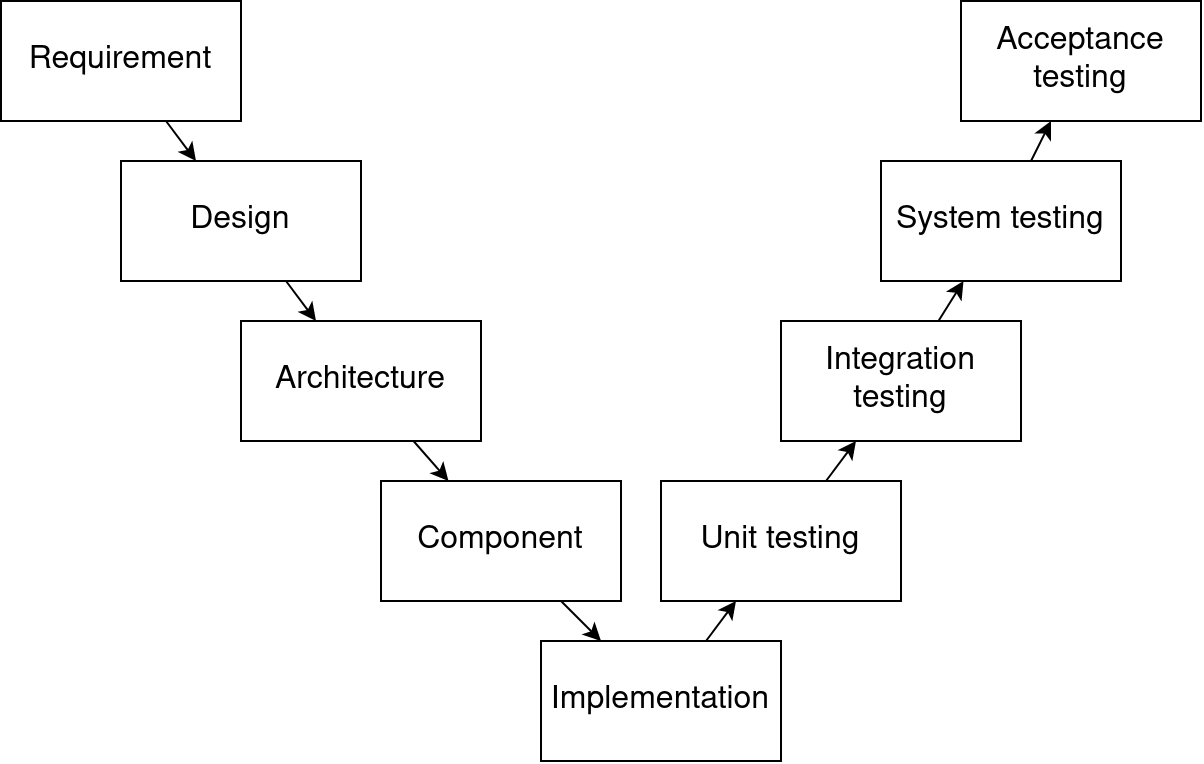
\includegraphics[width=0.5\textheight]{img/introduction/software-testing-v.drawio}
\caption{Levels of abstraction and their corresponding tests}
\label{fig:levels-of-abstraction-and-tests}
\end{figure}

Automated tests address the first issue.
Testing is well established and understood in software development.
In figure \ref{fig:levels-of-abstraction-and-tests}, different types of tests can be seen that correspond to different levels of abstraction of the system.
Single components are unit tested in isolation, while their interaction is tested using integration tests and so on and so forth.
In order to validate code before an automatic integration occurs, a well-founded set of tests is needed.
Not only on the lowest levels, but also on the highest level that is acceptance testing.
Without strong test suits,  faulty code may be integrated into the system and delivered to stakeholders.

For many systems, this is where the story ends.
Tests are designed and implemented.
The system grows so do its tests.
Everytime new code is written, tests are added, previous ones are run and the code is integrated.

The problem is solved.
Well, not entirely.
One small type of complex systems still holds out against the tests.
And life is not easy for the testers, who garrison the test suits of components, architecture, design and requirements \cite{AsterixBeginningSentence}.

These systems are those that run in clusters.
A collection of servers, varying in size, connected together fulfilling one or many business cases.
They exist and run in sometimes huge environments.
Lower level testing, such as unit testing, is not much different or different at all.
However, the higher level the testing is done the more complex, and resource intensive, testing becomes.
For example, to test such a system on the level of system testing, a cluster is needed for the system to run in.
Which in turn means setting up servers, connecting them to a cluster and installing management software, even before the first test can run.
After a test ran, this environment then needs to be destroyed and recreated, so that the next test can be run uninfluenced by the one that came before.

With great complexity comes a great learning curve.
Not all developers in a team might have the domain knowledge to create and maintain a pipeline configuration for such a setup.
Therefore, the first research question for this paper is the following.

Q1: How can the setup and maintenance of an environment for higher level tests be abstracted and made accessible?

The second problem after testing such highly complex systems is the delivery and distribution.
Usually, programs are delivered in the form of binaries, distributed often by a website or package management system.
As is shown later, distribution of cluster systems is highly diverse with many so-called ''marketplaces'' from which that software can be deployed from.
Targeting many of these systems multiplies the problem touched before, needing more changelogs, setting versions correctly and, additionally, adhering to proprietary configurations for specific marketplaces.
Henceforth, the second research question to be answered si as follows.

Q2: How can multiple distribution systems be integrated into an automatic pipeline using a common base of data and metadata.

\section{Structure}\label{sec:structure}

First it is discused, how those questions are going to be answered.
In other words, what methods are used and how they are evaluated.
Naturally, the specific technologies to implement these methods are also listed and described.

Next, scientific research that has already been done is discussed.
As is shown later, some of the implemented techniques are either theoretically discussed in other papers or were already used in a different context.
The context of this paper is explained afterwards.

The largest part then is 
the implementation.
What is theoretically disucssed in the beginning is later implemented practically as part of this thesis.
Details of this implementation are shown and explained.

Finally, the result of this thesis is evaluated.
A conclusion is then drawn from this evaluation.
